\chapter{Proposed Frameworks for Spatial-Temporal UAD}
\label{chap:sdm}

In this section, we introduce our proposed framework for Spatial-Temporal unsupervised anomaly detection, comprises two main modules: \ac{SDM} (\cref{sec:sdm}) and Anomaly Detection Module (\cref{sec:fam}). During the training of \ac{SDM}, we remove all temporal dependencies between samples and treat them as \emph{i.i.d} sample. \ac{SDM} accounts only for the spatial representations of the input. At inference, we add back the temporal dependencies using longitudinal module to increase the accuracy of anomaly segmentation. 

\minitoc

\section{Spatial Diffusion Model for pseudo-healthy data generation}
\label{sec:sdm}

\begin{figure}[htbp]
    \centering
    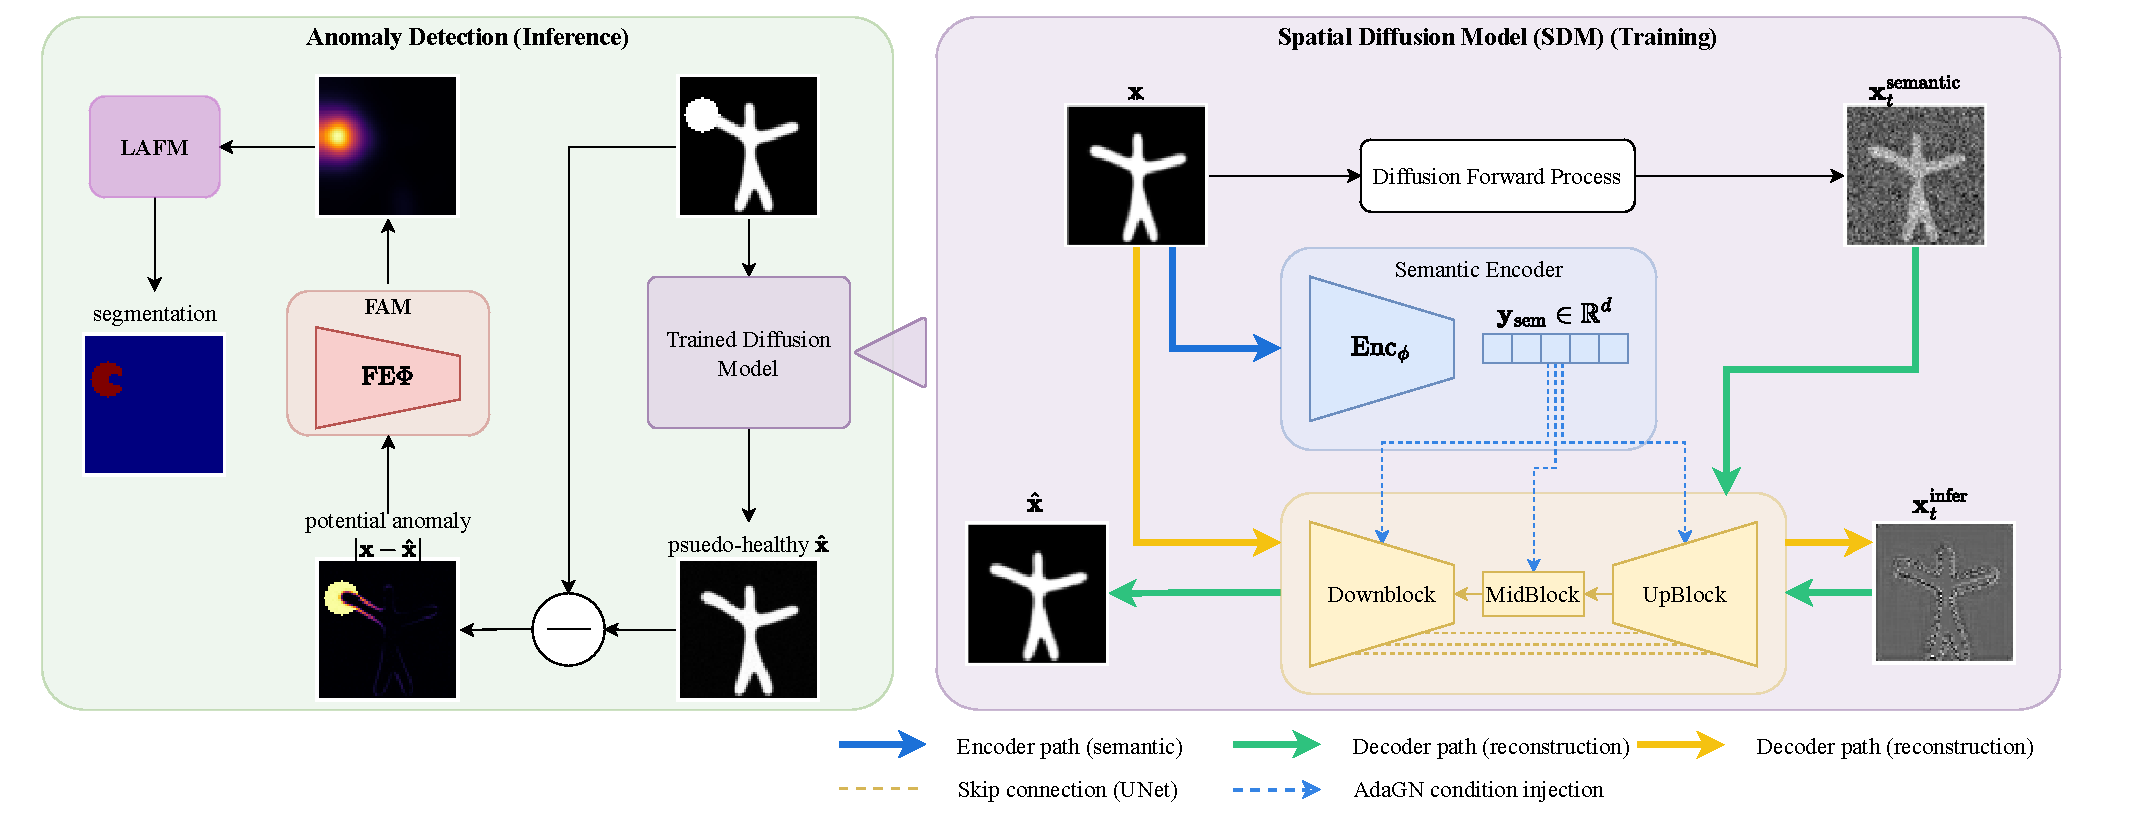
\includegraphics[width=1\linewidth]{figures/model-sdm.pdf}
    \caption[Overview of Spatial-Temporal UAD framework]{Overview of our \ac{SDM} framework for unsupervised anomaly detection using reconstruction-based method. Our model consists of four keys components: (i) \textbf{semantic encoder} extracts a non-spatial representation of input $(\rvx \to \rvy_{\text{sem}})$, (ii) \textbf{denoising UNet} comprises a down block, a middle block and up block with skip connection to concatenate information from down blocks to corresponding up blocks, (iii) \textbf{Feature Attention Module (FAM)}, and (iv) \textbf{Longitudinal Attention Fusion Module (LAFM)}. The semantic representation is injected as conditions into our diffusion process. Conditional diffusion UNet acts as both a stochastic encoder $(\rvx \to \rvx_T^{\text{infer}})$ and a decoder (DDIM denoising step) $(\rvx_T \to \widehat{\rvx})$. During inference, we use trained SDM to reconstruct pseudo-healthy image of input, and potential anomaly map is calculated as residual $|\rvx - \hat{\rvx}|$. We use \ac{FAM} to clean residual map, and \ac{LAFM} module further fuses information from other time points to have final anomaly segmentation.} 
    \label{fig:model-sdm}
\end{figure}

We now introduce the framework of our proposed SDM, with anomaly detection process during inference. Our SDM comprises four keys blocks: a semantic encoder (\cref{sec:method-semantic-encoder}), a denoising UNet (\cref{sec:method-unet}), a \ac{FAM} (\cref{sec:feature-extractor-network}) and a \ac{LAFM} (\cref{sec:method-lafm}). These four components, summarized in \cref{fig:model-sdm}, collectively can address the challenges we outlined in the introduction. We structure the description of SDM into two parts: this section provides a detailed explanation of diffusion model for image reconstruction (training phase). \cref{sec:fam} will discuss anomaly detection during inference phase. In training process, our SDM is designed as a conditional diffusion model that treats each $\rvx^i_l \quad (l = 1, ..., L_i)$ as independent cross-sectional data. To simplify the notation, we omit the superscript $i$ and subscript $l$ from here onward. During inference, we introduce \ac{FAM} and \ac{LAFM} after the denoising process to achieve final anomaly prediction and anomaly segmentation. 

\subsection{Semantic Encoder}
\label{sec:method-semantic-encoder}

The goal of the semantic encoder $\mathrm{Enc}_\phi(\rvx)$ is to summarize an input image into a meaningful non-spatial representation $\rvy_{\text{sem}} \in \mathbb{R}^d$ with enough information to help the decoder $p_\theta(\rvx_{t - 1}|\rvx_t, \rvy_{\text{sem}})$ denoise and predict the output image. We employ ResNet-50 \cite{ResNet50} as our semantic encoder. ResNet-50 has 50 layers, and is built around residual connections that enable stable training of very deep models. It comprises four main residual blocks operating at progressively lower spatial resolutions that capture hierarchical feature representations of the input. We replace the last classifier layer with an MLP that produces a non-spatial representation of the input. Together with time step $t$, $\rvy_{\text{sem}}$ form the condition that we will inject into diffusion UNet. 

\subsection{Diffusion UNet}
\label{sec:method-unet}

The core component of our SDM is denoising UNet module $\epsilon_{\theta}$ with trainable parameter $\theta$, adapted from \cite{dhariwalDiffusionModelsBeatGAN2021}. Given a clean image $\rvx$ and a time step $t$, we add noise to the image using \cref{eq:xt-from-x0}. The time step $t$ controls the amount of added noise and is sampled from $t \sim \mathrm{Uniform}(1 \ldots T )$. When $t=T$, the image $\rvx$ is transformed into pure noise $\rvx_T \sim \mathcal{N}(0, \mathbf{I})$. Subsequently, $\rvx_t$ is passed through the UNet, which predicts the added noise. We condition the backward process on context vector comprises time step and semantic representation $c=(t, \rvy_{\text{sem}})$. Time step is embedded using sinusoidal positional embeddings, originated from \cite{vaswani2023attentionneed}, while semantic representation is the output of our semantic encoder. To provide context $c$ into UNet, we use FiLM-style adaptive group norm (\textrm{AdaGN}), following \cite{dhariwalDiffusionModelsBeatGAN2021}. We formulate our \textrm{AdaGN} operation as: 
\begin{align}
    \mathrm{AdaGN}(\rvh, t, \rvy_{\text{sem}}) = \rvy_{\text{sem}}^s (\rvt_s . \mathrm{GroupNorm}(\rvh) + \rvt_b) + \rvy_{\text{sem}}^b \label{eq:adagn}
\end{align}
% To provide context, we use a semantic encoder to map the original image $\rvx$ to $\rvy_{\text{sem}} \in \mathbb{R}^d$, together with the corresponding time step $t$. The time step is embedded using sinusoidal positional embeddings. Both $t$ and $\rvy_{\text{sem}}$ are injected into the UNet via FiLM-style adaptive group normalization, following \cite{dhariwalDiffusionModelsBeatGAN2021}.

where $\rvh$ denotes the hidden feature map at each level of the UNet. The pairs $[\rvy_{\text{sem}}^s, \rvy_{\text{sem}}^b]$ and $[\rvt_s, \rvt_b]$ are obtained via linear projections of $\rvy_{\text{sem}}$ and $t$, respectively. They represent the \emph{shift} and \emph{scale} parameters applied to the feature maps, effectively adjusting them according to the conditioning signals. This design enables the model to guide the denoising process using high-level semantic codes. Compared to using a cross-attention module as in \cite{rombachLDM}, this approach is simpler, and unlike concatenating $\rvy$ with $t$ as in \cite{behrendt2025cDDPM}, it does not increase the hidden dimensionality of $\rvh$.

The semantic encoder is jointly trained with UNet with updated loss function: 
\begin{align}
    \mathcal{L} (\theta, \phi) &= || \epsilon - \epsilon_{\theta}(\rvx_t, t, \mathrm{Enc}_{\phi}(\rvx)||^2 \label{ep:loss-cond-encoder-ddpm}
\end{align}

We can interpret this training algorithm as forcing the semantic encoder $\mathrm{Enc}\phi$ to capture as much information about $\rvx$ as possible. Theoretically, if $\rvy_{\text{sem}} = \mathrm{Enc}\phi(\rvx) \in \mathbb{R}^d$ retains all the information of the input, we can achieve exact reconstruction \cite{lozuponeLDAE2025}. 

During inference, our trained model can generate a new sample by denoising process using \cref{eq:ddpm-sample}, starting from pure noise $\rvx_T \sim \mathcal{N}(0, \mathbf{I})$. We elevate the sampling process using DDIM sampling scheme, using \cref{eq:ddim-sample-deterministic}. We set $\sigma=0$ to have a deterministic process. It is worth noting that although the training process is performed with $T = 1000$ steps, it is not necessary to reconstruct healthy images from pure noise. In fact, since our main objective is not to generate entirely new images but rather to heal anomalous regions, it is preferable to start decoding from a noise level $t < T$. Using this approach, we preserve some high-level structure of the original image, in contrast to starting from pure noise. The noisy image $\rvx_t$ is obtained by adding noise to $\rvx_0$ with \cref{eq:xt-from-x0}.

\subsection{Stochastic Encoder and Conditional Decoder}

% As shown in \cite{DiffAE, lozuponeLDAE2025}
Here, we provide further insights into our encode and decode processes. We refer to our semantic encoder in \cref{sec:method-semantic-encoder} as \emph{semantic encoder}, which map input into its nonspatial representation. We will refer to $\rvy_{\text{sem}}$ as our \emph{semantic subcode}. In addition, our denoising network $\epsilon_\theta$ plays a dual role in our model. Its main purpose is to act as a \emph{conditional decoder} that can generate healthy images from noisy input. On the other hand, it can also serve as a \emph{stochastic encoder} by using deterministic DDIM sampling scheme. Given a clean image $\rvx$, SDM can encode it to a stochastic subcode using \cref{ep:ddim-encode}. \cite{DiffAE, lozuponeLDAE2025} demonstrates that this stochastic subcode contains fine grain details about $\rvx$ that is not captured by semantic encoder. We note that, unlike the standard noising process \cref{eq:xt-from-x0}, the stochastic subcode does not necessarily follow Gaussian noise, since it retains residual information about the input. We refer to \emph{stochastic subcode} of original image $\rvx$ as $\rvx_t^{\mathrm{infer}}$, and normal noisy image as $\rvx_t^{\textrm{semantic}}$ (or $\rvx_t$) \footnote{We note that in our report, $\rvx_t^{\text{semantic}}$ and $\rvx_t$ are used interchangeably. $\rvx_t^{\text{semantic}}$ is used in the context of comparison with $\rvx_t^{\text{infer}}$ to emphasize the differences, whereas $\rvx_t$ is used elsewhere for the sake of brevity.}, with $t \leq T$. 

% \subsection{Anomaly Detection with SDM}
\section{Unsupervised Anomaly Detection Module}
\label{sec:fam}

% However, this approach faces several challenges when we have to deal with subtle anomaly. First, we will almost never achieve a perfect reconstruction even with healthy images, and the \textit{l1}-distance at pixel level rarely reachs $0$. This often results in false negatives, especially along sharp edges of objects. Second, pixel-wise comparisons can lead to false positives when slight distortions appear in the background, that the UNet model may not learn during training, and hence does not reconstruct accurately during inference. 

In the simplest case, reconstruction-based method relies on pixel wise difference between the original image $\rvx$ and psuedo-healthy reconstructed image $\hat{\rvx}$ to generate the anomaly map, which will be used as our anomaly segmentation. To address the challenges mentioned in \cref{sec:introduction-sdm}, we aim to employ techniques that: (i) ignore small outliers in the background, (ii) discard minor reconstruction errors around object edges, and (iii) emphasize differences within the critical anomaly region (i.e., the region of interest). \cite{zhang2018unreasonableeffectivenessdeepfeatures} introduce the effectiveness of using image features as perceptual metrics, which are robust to minor pixel-level differences that do not alter the overall image structure. Features are sensitive to changes in texture and shape, but can be robust against slight transformation where pixel level distance might fail. We follow method of DDAD \cite{DDAD} that defines anomaly score as combination of both pixel and feature errors. By utilizing both pixel differences and features differences, we can achieve high precision in anomaly localization. We refer to this process that wraps around the feature extractor network as our \ac{FAM}. We discuss the methodology of \ac{FAM} in the section below. 

%Based on this reasoning, PatchCore \cite{PatchCoretotalrecall} introduce anomaly score system that is entirely relies on feature distances. It uses locally aware patch features to build a memory bank of reference features extracted from healthy images. While PatchCore achieves state-of-the-art performance with $99.1\%$ AUROC without pixel level erros,  we think they are still good indicators for anomaly localization. 

\subsection{Feature Attention Module}
\label{sec:feature-extractor-network}

\paragraph{Anomaly score as combination of feature distances and pixel distances} Given an input image $\rvx$, and it's psuedo-healthy reconstruction $\hat{\rvx}$, we define a pixel-wise distance function $D_p$ and a feature-wise distance function $D_f$ to derive the anomaly heatmap. $D_p$ is calculated based on the $\gL_1$ norm in pixel space. At the feature level, we use adaptive average pooling to spatially smooth each individual feature map. Feature distance $D_f$ is then calculated as a cosine-similarity. Formally we have: 
\begin{align}
D_p(\rvx, \hat{\rvx}) &= \mathcal{L}_1(\rvx - \hat{\rvx}) \\
D_f(\rvx, \hat{\rvx}) &= \sum_{j \in J} \operatorname{Interp}\left(1 - \cos\left(\Phi_j(\rvx), \Phi_j(\hat{\rvx})\right)\right)
\end{align}

where $\Phi$ is a pre-trained feature extractor network and $j$ refers to the level (or stage) that we want to extract feature from, and $\operatorname{Interp}$ is the interpolation operator of feature maps to match input's resolution. We note that for each feature level $j$, the cosine similarity is calculated along channel dimension and for each pixel. Formally, we have $\rvx, \hat\rvx \in \mathbb{R}^{h \times w}$, $\Phi_j(\rvx), \Phi_j(\hat\rvx)$, and $\mathrm{cos}(., .) \in \mathbb{R}^{h_j \times w_j}$, with $h_j, w_j$ are dimensions of feature map $j$. 

We utilize our trained semantic encoder $\mathrm{Enc}_{\phi}$, and we train a copy of it as feature adaptation step. We give detail about this step in section \ref{sec:feature-extractor-network}. We follow the convention with existing literatures for ResNet-like architecture, so that $j \in \{1, 2, 3, 4\}$ indicating the final output of respective spatial resolution blocks. The final anomaly score (pixel wise) will be given as \cite{DDAD}: 
\begin{align}
    \rvs = D_\textnormal{anomaly} (\rvx, \hat{\rvx}) = \left( v \cdot D_p + D_f \frac{\max(D_p)}{\max(D_f)} \right)
\end{align}

where $v$ is the parameter to control the importance of the errors at pixel level, $D_{\textnormal{anomaly}}(., .) \in \sR^{h \times w}$ is spatial representation that retains the same height and width as the input, allowing for pixel-wise localization of anomalies. We use notation $\rvs$ to denote pixel-wise anomaly score map.  

% The feature extractor network $\Phi$ can be initialized using any pre-trained CNN model that provides hierarchical feature representations. However, these models are typically trained on generic datasets (e.g., ImageNet) and may not adapt well to the domain-specific characteristics of anomaly detection tasks or particular object categories. 
\paragraph{Feature Extractor Network}: is a trainable model \textrm{FE} with parameter $\Phi$. Following DDAD method \cite{DDAD}, \textrm{FE} is initialized from our semantic encoder $\mathrm{Enc}_{\phi}$, which is already jointly trained with conditioned diffusion UNet. Although it is trained specifically on our dataset to capture high semantic structure of input, it serves a slightly different purpose compared to $\Phi$. $\mathrm{Enc}_{\phi}$ is used to compress and capture as much information as possible about $\rvx$ to use as guidance in our diffusion process, while $\Phi$ needs to be trained to ignore discrepancies between $\rvx$ and $\hat{\rvx}$ that are not semantically meaningful. We train an extra step by converging different extracted layers from two nearly identical images.

Given an input $\rvx$ and a trained denoising model $\epsilon_{\theta}$, we go through a complete inference process of $\rvx \to \rvx_{T} \to \hat{\rvx}$ to create its reconstruction image. We then extract their features from $\Phi$, denoted as $\Phi_j (\rvx)$ and $\Phi_j (\hat{\rvx})$ respectively. Since we train the network on healthy training dataset only, we can make assumption that $\hat{\rvx} \sim \rvx$, thus their features should be similar. Therefore, our network $\Phi$ is fine-tuned by minimizing the distance between extracted features. We use cosine-similarity as our loss function, which is calculated for each of the final activation layers of the $j$th spatial resolution block. Similarly to \cite{DDAD}, we incorporate a distillation loss from a frozen feature extractor $\bar\phi = \textnormal{Enc}_{\phi}$ as a safeguard mechanism to prevent the network from losing its generalization it has been trained before. Formally, our loss function can be expressed as: 

\begin{align}
\gL_{\textnormal{sim}} &= \sum_{j \in J} \left( 1 - \cos\left(\Phi_j(\hat{\rvx}), \Phi_j(\rvx)\right) \right) \notag \\
&\quad + \lambda_{DL} \sum_{j \in J} \left( 1 - \cos\left(\Phi_j(\hat{\rvx}), \bar{\phi}_j(\hat{\rvx})\right) \right) \notag \\
&\quad + \lambda_{DL} \sum_{j \in J} \left( 1 - \cos\left(\Phi_j(\rvx), \bar{\phi}_j(\rvx)\right) \right) \label{eq:fe-dl-loss}
\end{align}

where $\lambda_{DL}$ controls the strength of our distillation losses. This network $\Phi$ will help to transfer the trained semantic encoder $\textnormal{Enc}_{\phi}$ to feature-distance network $\Phi$. Similar to \cite{DDAD, PatchCoretotalrecall} we set $j \in J = \{2, 3\}$, we only consider middle-sized blocks in our ResNet to retain the generality of the used features.

\subsection{Longitudinal Attention Fusion Module}
\label{sec:method-lafm}

\begin{figure}[htbp]
    \centering
    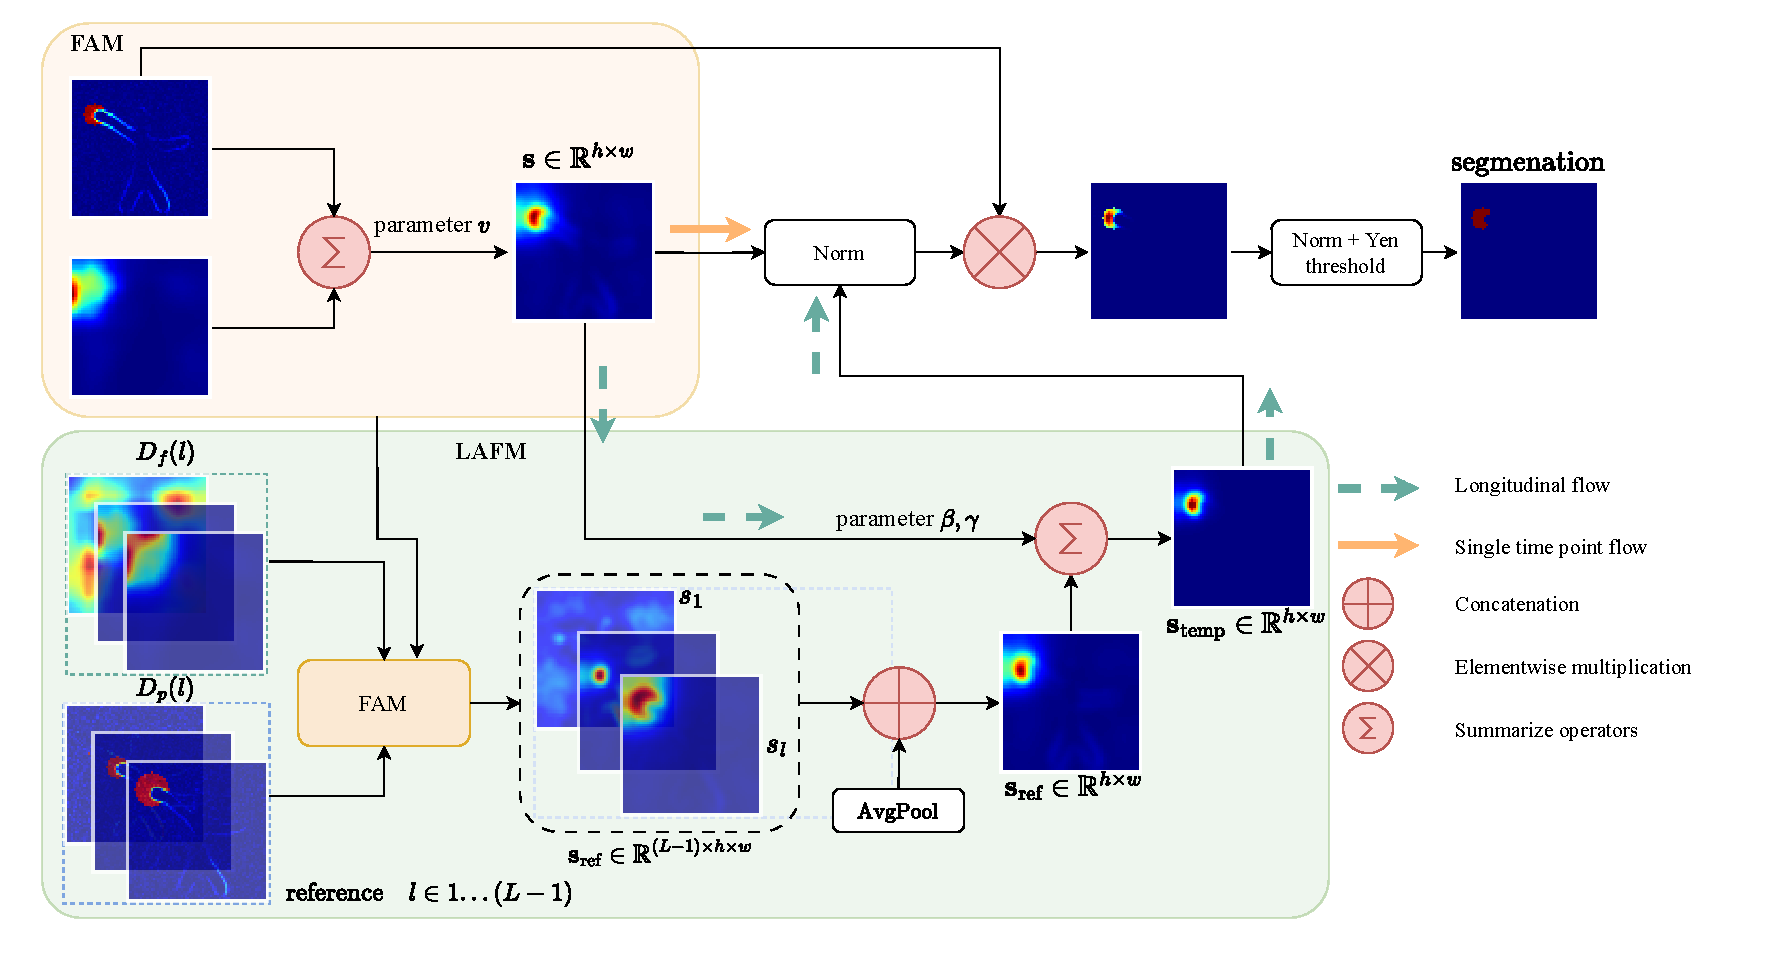
\includegraphics[width=0.95\linewidth]{figures/model-fam-lafm.pdf}
    \caption[Overview of FAM and LAFM module]{The overall structure of Feature Attention Module and Longitudinal Attention Fusion Module. For single time point (\textcolor{orange}{orange arrow}), anomaly segmentation is calculated directly from the output of FAM. With longitudinal data (\textcolor{green}{green arrow}), each time point anomaly score map is processed by FAM, concatenated together and applied the $F_{\text{mean}}$ operator with Gaussian weights (\cref{eq:laf_fusion}). The referenced anomaly score map $\rvx_{\text{ref}}$ is used to update the targeted anomaly score to have $\rvs_{\text{temp}}$ (\cref{eq:temp-smooth})}. 
    \label{fig:model-fam-lafm}
\end{figure}

Up to now, we have considered each sample as an i.i.d. draw from $p(\rvx)$. After combining feature distances and pixel distances from \cref{sec:feature-extractor-network}, each image $\rvx_0$ is associated with an anomaly score map $\rvs^{pixel} \in \mathbb{R}^{h \times w}$ that ideally contains sufficient information to determine which pixels are anomalous. Unfortunately, this is often not the case: if we detect anomalies independently at each time point, the anomaly score map can be noisy and exhibit: (i) false positives that appear at one time and then vanish, and (ii) missing of real anomalies (false negatives), especially when the anomalies are subtle. We assume that, in reality, anomalies usually have temporal persistence: they do not appear and disappear randomly\footnote{This might not be the case for patients undergoing treatment, but this scenario requires a different type of model and is beyond the scope of our experiment.}. Similar to \cite{wangEPDiffErasurePerception2025}, we design our \ac{LAFM} that acts as a temporal filter, enforcing the persistence of anomalies and smoothing out noise. We note that, in principle, our \ac{LAF} module is similar to the MAF module in \cite{wangEPDiffErasurePerception2025}, but instead of attending to information from multiple modalities at the same time point, here we concatenate information from a single modality across different time points. \cref{fig:model-fam-lafm} shows the overall structure of LAFM. 

We consider the full set of images collected for each patient, 
\[
\mathbf{X}_i = \{\rvx_1, \rvx_2, \dots, \rvx_L\}, \quad \rvx_l \in \mathbb{R}^{h \times w}, \quad l \in [1, \dots, L],
\] 
where $\rvx_l$ represents an image at a single time point $l$. Different patients may have a different total number of visits and images acquired at different time points. All images in the set $\mathbf{X}_i$ are processed through our \ac{SDM} model and \ac{FAM} as described above, yielding a corresponding set of anomaly score maps, 
\[
\mathbf{S}_i = \{\rvs_1, \rvs_2, \dots, \rvs_L\}.
\] 
We denote $\rvx$ as the target image and $\rvs$ as its corresponding anomaly score map at target time point $l_{\textnormal{target}}$. We further define the reference set 
\[
\rvs_{\text{ref}} = \mathbf{S}_i \setminus \{\rvs\}
\] 
as the set of anomaly score maps from other time points, excluding the target. Note that the length of $\rvs_{\text{ref}}$ is $L - 1$, and $\rvs_{\text{ref}} \in \mathbb{R}^{(L-1) \times h \times w}$.

Similar to MAF from \cite{wangEPDiffErasurePerception2025}, the role of \ac{LAFM} is to perform the weighted fusion of complementary information from reference time points, and ultimately to obtain the accurate anomaly masks. To fuse key information across time points and align it into a single output, we apply pixel-wise average pooling with a receptive field of 1. This gives us our mean response map $F_{mean}$ To account for the relative importance of each reference time point with respect to the target time point, we weight the reference anomaly score maps using a Gaussian kernel. Formally, we have: 

% We first concatenate all $\mathbf{S}_{\textnormal{ref}}$ together to obtain $\rvs_{\textnormal{ref}} \in \mathbb{R}^{(L-1) \times h \times w}$. 

\begin{equation}
\label{eq:laf_fusion}
\begin{aligned}
    \rvs_{\text{ref}} &= \oplus \{\rvs_l\}, \quad l \in [1, \dots, L], \; l \neq l_{\text{target}} \\
    \rvw &= \exp\Bigg(-\frac{(\rvl - l_\text{target}\mathbf{I})^2}{2\sigma^2}\Bigg) \\
    F_{\text{mean}} &= \mathrm{AvgPool}(\rvs_{\text{ref}} \odot \rvw) \in \mathbb{R}^{h \times w} 
\end{aligned}
\end{equation}

where 
\begin{itemize}
    \item $\mathbf{l} = [\, l_1, l_2, \dots, l_L \,]^\top$ is the vector of reference time points.
    \item \(l_\text{target}\) is the target time point.  
    \item \(\mathbf{w} = [\, w_1, w_2, \dots, w_L \,]^\top\) is the vector of Gaussian weights. 
    \item \(\sigma\) controls the temporal decay rate.
    \item $\oplus$ denotes concatenation and $\odot$ denotes element wise multiplication. 
\end{itemize}

Finally, we combine $\rvs_{\textnormal{ref}}$ with target anomaly score $\rvs$ using: 
\begin{align}
    \rvs_{\text{temp}} &= \underbrace{\rvs \times (1 - \beta \times (1 - \mathrm{Norm}(\rvs_{\text{ref}})))}_{\text{eliminate false positive}} + \underbrace{\gamma \times \rvs_{\text{ref}}}_{\text{eliminate false negative}} \label{eq:temp-smooth}
\end{align}

We refer to this as \emph{temporal smoothing operation} of $\rvs$, and it can be interpreted as follows: first, we normalize $\rvs_{\text{ref}}$ using min-max normalization. This transforms raw anomaly score into the scaled anomaly probability at each pixel. The first expression of RHS of \cref{eq:temp-smooth} is to eliminate false negative in target image. For example, if pixel $p_{i, j}$ is flagged as anomalous in $\rvs$, we check to see if it is consistent over time period. If this is a false positive, meaning this is pixel error cause by reconstruction process, it will not persist over time and thus its reference value across time will be small, i.e. $p_{i, j}^{\text{ref}, \text{norm}} \approx 0$. We negate its value and subtract it from $\rvs$, efficiently reducing its anomaly score. We note that here we are working with normalized scaled anomaly score $(1 - \mathrm{Norm}(\rvs_{\text{ref}})) \in [0, 1]$, so the target score will be scaled down according to its reference. Conversely, if the error persists over time, its reference value will be higher $p_{i, j}^{\text{ref}, \text{norm}} \approx 1$, and in this case we keep it unchanged. $\beta \in [0, 1]$ is hyperparameter controls how much the reference information influences the final anomaly score. In our setting, we choose $\beta = 1$ to strictly limit false positive, because in our experiments we observed that our model performs well in detecting anomalies, but tends to produce false positives on small pixel errors in healthy data. The second expression on the RHS of \cref{eq:temp-smooth} helps to decrease false negative. In particular, if a pixel $p_{i, j}^{\text{ref}, \text{norm}}$ is consistently flagged as anomalous across reference time points, but our model is false to detect in the current anomaly score map $\rvs$, we want to increase its value $p_{i, j}$. Hyperparameter $\gamma$ controls how much information is incorporated from $\rvs_{\text{ref}}$ to $\rvs$. As note earlier, false negatives are not a major issue in our model, so we set a relatively small $\gamma = 0.1$ as a safeguard mechanism. 

\subsection{Post Processing}
\label{sec:post-process}
\begin{description}
    \item[Pixel anomaly score]: We adapt some common post-processing technique used in UAD domain to further clean the residual map $\rvs_{l}$ before binarizing it to obtain anomaly segmentation \cite{behrendt2025cDDPM, baur_autoencoders_2020}. First, we apply a median filter with kernel size $k_{mf} = 5 \times 5$ to smooth out the anomaly score map, and to reduce the influence of noise to obtain a more reliable distribution of the anomalies. Next, we apply min–max normalization on a per-patient basis. This differs from other methods (cDDPM \cite{behrendt2025cDDPM}, EPDiff \cite{wangEPDiffErasurePerception2025}) where the authors apply normalization at each image/volume individually. 
    % By grouping all images from a single patient and performing the operation jointly, we provide more informatioachieve a more accurate separation between anomalous and healthy pixels. 
    \item[Pixel anomaly segmentation]: To obtain the localization of anomalies, a binary map is obtained by thresholding the anomaly score map. In previous methods \cite{autoDDPM, behrendt2025cDDPM, DDAD}, the optimal threshold for segmentation was found using a greedy search strategy on the validation dataset, by calculating the AUPRC metric and find the best theoretical value. However, ground truth annotations need to be provided in order to perform these search, and we argue that using labeled data will compromise the unsupervised setup (\cref{sec:introduction-sdm}). We follow \cite{wangEPDiffErasurePerception2025} to employ Yen threshold technique \cite{YenThreshold}, which is an automatic image thresholding strategy that can separate background and foreground based on histogram of gray levels in the image. We can formulate our whole post-processing for pixel anomaly score as follows: 
    \begin{equation}
    \label{eq:post-process-pixel}
        \begin{aligned}
            \mathbf{S}_{\text{temp}} &= [\rvs_{\text{temp},1}, \rvs_{\text{temp},2}, \dots, \rvs_{\text{temp},L}] \\
            \mathbf{S}_{\text{temp}} &= \mathrm{Norm} (\mathrm{MedianFilter}(k_{mf})(\mathbf{S}_{\text{temp}})) \\
            \text{thres} &= \mathrm{YenThreshold}(\mathbf{S}) \\
            \text{m}_{i, j} &= 
            \begin{cases}
            0 & \text{if } s_{i,j} < \text{thres} \\
            1 & \text{if } s_{i,j} \geq \text{thres}
            \end{cases} \\
            \mathbf{D}_{p} &= \text{m} \odot \mathbf{D}_p \\
            \text{p\_thres} &= \mathrm{YenThreshold}(\mathbf{D}_p) \\
            \text{p\_m}_{i,j} &=
            \begin{cases}
            0 & \text{if } d_{i,j} < \text{p\_thres} \\
            1 & \text{otherwise}
            \end{cases} \\
            \text{ano\_m} &= \text{m} \cap \text{p\_m}
        \end{aligned}
    \end{equation}

    where $\mathbf{S} \in \mathbb{R}^{L \times h \times w}$ is batch of all anomaly score maps (updated from LAFM) for 1 patient $i$, and $\mathbf{D}_p \in \mathbb{R}^{L \times h \times w}$ is batch of all pixel distance maps. Here we drop the subscript $i$ for brevity. $\text{m}$ and $\text{p\_m}$ are anomaly score segmentation maps and pixel distance segmentation maps, respectively. The final anomaly segmentation maps are defined as intersection between the twos. 
    
    \item[Image anomaly score]: After post-processing step, we obtain the pixel-level anomaly score $\rvs \in \mathbb{R}^{h \times w}$ for each individual image. For image-level anomaly score, a common practice in the literature is taking the mean over all pixel values in the anomaly map. \cite{DDAD, lagogiannisUnsupervisedPathologyDetection2024} use the maximum value across pixels and assign it as the overall anomaly score of the image, with the argument that it should be independent of the anomaly size. \cite{wuUADPostSampling2024} combine both technique and design the image-wise anomaly score as the average of the largest $S$ pixel wise anomaly scores in $\rvs$ to mitigate false positives caused by image noise. We employ several similar techniques, which will be discussed in \cref{sec:image-auprc-auroc}.
\end{description}



% There are some common post-processing technique irst, we apply a median filter with kernal size of $K = 5 \times 5 \times 5$ to smooth the residual map. Next, we perform barin mask eroding for 3 iterations to filter out pixel differences caused by poor reconstructions along the sharp edge of the object. Finally, the binary segmentation map $\rvm \in \sR^{h \times w}$ is obtained by thresholding the post-processed residual map $\rvr \in \sR^{h \times w}$, using $m_{i, j} = 1$ if $\rvr_{i,j} > \mathrm{threshold}$, otherwise $m_{i, j} = $. As a final step, following the method of \cite{behrendt2025cDDPM}, we use connected component filtering to remove areas that include less than 7 voxels. In this step, we can make use of domain-specific knowledge to further remove false-positive predictions that are smaller than the anomalies considered in our study.  

% \subsubsubsection{Some other post-processing technique}

% \begin{description}
%     \item[\href{https://hal.science/hal-02995591/file/Papier_MEDIA_Alaverdyan_2020.pdf}{Regularized siamese autoencoder for UAD in MRI}]: 3 steps techniques that first normalizing the distance maps with respect to the intra-subject spatial variability. For that purpose, the distance maps of the control subjects are computed by performing a k-fold evaluation of the training set (i.e. for each fold of normal subjects, the distance maps are obtained with oc-SVMs trained on the remaining subjects). The second step is to pool all pixel-wise distance into a histogram and estimate the distribution with non-parametric method (kernel density estimation). 26 connectivity then used to define cluster. Finally, the third step consists in ranking the cluster. 

%     \item[\href{https://hal.science/hal-03962874v1/document}{Voxel based OC-SVM}]: perform Oc-SVM at each pixel/voxel, i.e each voxel will fit 1 OC-SVM model. Each voxel is represented by a feature vector $\mathbf{V}^d$ with ($d=2$), so OC-SVM is trained with $n$ vector of 2 dimensional. Given a test sample we will obtain a OC-SVM distance map by trained OC-SVM models for each voxel, we will use the raw score as OCSVM map. thresholding this score map is done by modeling the probability distribution of the OC-SVM scores for normal voxel. This normative score distribution was computed by performing a leave-one-out procedure on the normal subjects (or we can use $k-$fold strategy). Assuming we obtain $k$ score map (on healthy training dataset), $k$ corresponding histograms are calculate with the same bin width and value range, normative histogram is obtained by averaging all $k$ histogram. This distribution was then approximated by a non-parametric distribution using a kernel density estimator to convert score values into probability density estimates. We assume that the OC-SVM score distribution of any given test patient can be represented by this normative score distribution, except those are inside anomaly region which we can consider to be outlier of the distribution. The type I error can then be controlled by using a threshold value that corresponds to a given $p-$value on the normative distribution. 
%     The clustering process then consists in scanning the thresholded map in a lexico-graphical voxel order and aggregating all non-null voxels that are linked for the 26-connectivity rule. Descriptive statistics per cluster (size, minimum, maximum and mean of the voxel scores) are then computed. Each cluster is assigned a value that corresponds to the minimum OC-SVM score value of its constituting voxels, i.e. the smallest probability value of belonging to the normal class. Finally, a labelled cluster map is generated in which cluster order is given by the minimum (i.e. most pathological) OC-SVM score value.
% \end{description}

% \subsubsection{Pixel anomaly score and Image anomaly score}

% After post-processing step, we obtain the pixel-level anomaly score $\rvr \in \sR^{h \times w}$. For image-level anomaly score, a common practice in the literature is taking the mean over all pixel values in the anomaly map. \cite{DDAD, lagogiannisUnsupervisedPathologyDetection2024} use the maximum value across pixels and assign it as the overall anomaly score of the image, with the argument that it should be independent of the anomaly size. \cite{wuUADPostSampling2024} combine both technique and design the image-wise anomaly score as the average of the largest $S$ pixel wise anomaly scores in $\rvr$ to mitigate false positives caused by image noise. 

% \subsubsection{Anomaly threshold}

% In the field of UAD for medical images, selecting an appropriate threshold remains a critical and ongoing challenge—both for binarizing the anomaly score map to obtain pixel-level anomaly segmentation, and for assigning a single class label at the image level. 

% \subsection{One Class SVM}

% Reference from paper: \href{https://hal.science/hal-05164029/document}{OVSVM guided autoencoder for UAD}
% \\
% The dual form of OCSVM is as follow: 
% \begin{align}
%     \min_{\alpha} \frac{1}{2} \sum_{i=1}^{n}\sum_{j=1}^{n} \alpha_i \alpha_j k(\rvz_i, \rvz_j) \\
%     \text{subject to: } 0 \leq \alpha \leq \frac{1}{\nu n} \quad n \in [1, n] \notag \\
%     \sum\alpha_i = 1 \notag
% \end{align}

% OCSVM is solved using \texttt{cvxpy} package, in which we optimize over $\alpha^*$ with fixed kernel $K$. However, in the coupled setting we integrate our function into our neural network, and $K$ depends on the latent variable $\rvz_i$. The optimization problem ( \verb+CvxpyLayer+) solves for $\alpha$, but the loss depends on how the features $\rvx_i$ produce a good decision boundary.
% Backpropagation flows through the solution of the \verb+CVXPY+ problem (through the optimzed $\alpha*$ values), back to the parameters $\theta$ of our network. For this reason, we indirectly optimize $K$ using OCSVM. 

% \verb+CVXPY+ must recognize the problem as \emph{disciplined convex programming} (DCP) compliant, and we cannot have parameters appear in quadratic form. We utilize the fact that $K$ is positive semi-definite (a gram matrix) to rewrite the problem as: 
% \begin{align}
%     K &= K^{\frac{1}{2}T} K^{\frac{1}{2}} \\
%     \bm{\alpha}^TK \bm\alpha &= \bm\alpha^T K^{\frac{1}{2}T} K^{\frac{1}{2}} \bm\alpha \\
%     \bm{\alpha}^TK \bm\alpha &= \|K^{\frac{1}{2}}\bm\alpha\|^2
% \end{align}

% \subsubsection{OCSVM for Image-wise anomaly score}

% We will train our OCSVM model on semantic encoder output $\rvy_{\text{sem}} = \mathrm{Enc_{\phi}(\rvx)}$, based on the assumption that after diffusion training, $\rvy_{\text{sem}}$ captures the most important features of our input and can be use to generate new sample that shares the same structure as input. We also utilize OCSVM step to further reduce the dimension of $\rvy_{\text{sem}}$ for downstream task of longitudinal learning, thus we include a small autoencoder network in OCSVM $\rvz_{\text{sem}} = \mathcal{E}(\rvy_{\text{sem}})$ and OCSVM will learn the decision boundary on these latent variabls instead of directly on $\rvy_{\text{sem}}$. To minimize the underlying rank of $\rvz_{\text{sem}}$, we follow the method of \href{https://arxiv.org/abs/2010.00679}{implicit rank-minizing autoencoder} by adding $l$ linear transformation matrices between encoder and decoder. The latent variable $\rvz_{\text{sem}}$ becomes: 

% \begin{equation}
%     \rvz_{\text{sem}} = \mathcal{D}(W_l \dots W_2 W_1 \mathcal{E}(\rvy_{\text{sem}}))
% \end{equation}

% \textbf{Main idea of the paper}: a series of linear matrices $W_l \dots W_2 W_1$ form a linear neural network between the encoder and decoder, acting as an implicit regularization. During training, these matrices encourage latent variables to use a lower number of dimensions and effectively minimize the rank of covariance matrix of the latent space. Each $W_i \quad i \in [1 \dots L]$ is a square matrix that does not change the dimension between input and output. We note that these matrices are equivalent to a single linear layer at inference time, and thus they do not change the capacity of the autoencoder. 

% IRMAE \href{https://github.com/facebookresearch/irmae/blob/main/model.py}{github}

